

\documentclass[conference]{IEEEtran}
\IEEEoverridecommandlockouts

\usepackage{cite}
\usepackage{amsmath,amssymb,amsfonts}
\usepackage{algorithmic}
\usepackage{graphicx}   
\usepackage{textcomp}
\usepackage{xcolor}
\usepackage{amsmath}
\usepackage{subcaption}
\usepackage{url}
\usepackage{booktabs}
\usepackage{multirow}
\usepackage{makecell}
\usepackage[table]{xcolor}
\usepackage{array}
\usepackage{hhline}
\usepackage{comment}

\usepackage[top=0.75in, bottom=1in, left=0.625in, right=0.625in]{geometry}

\definecolor{cfire}{HTML}{d62728}
\definecolor{cnofire}{HTML}{2ca02c}
\definecolor{cefire}{HTML}{ff7f0e}
\definecolor{cenofire}{HTML}{1f77b4}
\newlength{\sampleimgw}
\newcommand{\smplimg}[2]{%
  {\setlength{\fboxsep}{0.8pt}\setlength{\fboxrule}{0.5pt}%
   \fcolorbox{#1}{white}{\includegraphics[width=\sampleimgw]{sample_images/#2}}}}

\def\BibTeX{{\rm B\kern-.05em{\sc i\kern-.025em b}\kern-.08em
    T\kern-.1667em\lower.7ex\hbox{E}\kern-.125emX}}

\title{Cross-Domain Generalization of Deep CNN Architectures for Fire Detection: A Multi-Resolution Benchmark with Mixed-Precision Inference}


\author{

    \IEEEauthorblockN{Muhammad Talha\IEEEauthorrefmark{1}, Syed Muhammad Hamza Tauqeer\IEEEauthorrefmark{2}, Huma Ghafoor\IEEEauthorrefmark{1}
        }
    \IEEEauthorblockA{\IEEEauthorrefmark{1}School of Electrical Engineering and Computer Science (SEECS),\\National University of Sciences \& Technology (NUST), Pakistan\\ \IEEEauthorrefmark{2} Military Collge of Signals (MCS), National University of Sciences \& Technology (NUST)}
    \IEEEauthorblockA{Email: \{mtalha.bee20seecs, huma.ghafoor\}@seecs.edu.pk, stauqeer.msee24mcs@student.nust.edu.pk}
}
\begin{document}
\maketitle


\begin{abstract}
Convolutional neural networks (CNNs) are routinely reported at near-perfect accuracy for image-based fire detection, but almost always on test data drawn from the training distribution, so their reliability under domain shift remains largely unmeasured. We benchmark ten CNN architectures for binary fire/no-fire classification across two distinct domains, training on a wildfire dataset and testing on an independent forest fire dataset. Each model is trained at three input resolutions (32$\times$32, 64$\times$64, and 128$\times$128\,px) over five random seeds (150 configurations in total), and timed for per-image FP16 inference under automatic mixed precision on an RTX~5090 GPU. Internal and external performance diverge sharply: models within 0.5 points of one another on internal validation separate by far more on the external domain, with MobileNet-V3-Large losing 15.7 points. DenseNet-121 transfers best, reaching 84.99$\pm$2.48\% external accuracy and 92.51\% ROC-AUC, whereas ResNet-18 at 32$\times$32 is fastest at 0.0354\,ms per image and 80.81\% accuracy. The gain from higher resolution is architecture-dependent, and per-seed AUC variance exposes instability that mean accuracy conceals. We argue that external-domain testing, multi-resolution analysis, and FP16 latency belong in any fire-detection benchmark, and we give concrete model-selection guidance for accuracy- and latency-driven deployment.
\end{abstract}

\begin{IEEEkeywords}
Accuracy--latency trade-off, convolutional neural networks, cross-domain generalization, domain shift, fire detection, mixed-precision (FP16) inference, multi-resolution analysis, transfer learning.
\end{IEEEkeywords}


\section{Introduction}

Forest fires, or wildfires, threaten ecosystems, human settlements, infrastructure, and biodiversity. Recent events such as the 2025 Los Angeles wildfires and the 2019--2020 Australian bushfires show how quickly an uncontrolled fire can spread and how lasting its ecological and economic damage can be~\cite{fitzgerald2025wildfires, wikipedia2025bushfires}. Because the cost of a fire rises sharply with the time it goes undetected, early and reliable detection is essential for shortening response times and limiting false alarms. Computer vision and deep learning have consequently become central to automated fire monitoring, especially on unmanned aerial vehicles (UAVs), remote-sensing platforms, and edge surveillance systems~\cite{saleh2024review, gonccalves2024wildfire, mu2025edge, abdusalomov2025ai}.

Recent fire-detection research has advanced along two lines. The first pursues accuracy through specialised object detectors, including dual-channel and attention-guided YOLO variants~\cite{he2024dcgc, yu2025improved}, improved YOLOv8 smoke detectors~\cite{zhang2024research}, and transformer detectors for embedded platforms~\cite{zheng2024fta}. The second pursues efficiency through vision transformers and attention-augmented lightweight models~\cite{kluska2024qattn, bukhari2025irtq}. Pure vision transformers, however, need far more training data and run slower per image on embedded and UAV hardware than convolutional models~\cite{kluska2024qattn}. The quantized hybrid of Bukhari~et~al.~\cite{bukhari2025irtq} reaches competitive accuracy but is tested on a single dataset, without cross-domain validation or multi-resolution analysis. Similarly, the hybrid YOLOv4--EfficientNetV2 detector of Mamadmurodov~et~al.~\cite{mamadmurodov2025hybrid} reports strong precision on curated data but no FP16 latency or external-domain results. Convolutional neural networks (CNNs) thus remain the practical choice for latency-sensitive edge deployment, yet their behaviour under mixed-precision inference and domain shift has not been benchmarked across input resolutions.

Hardware-aware optimisation matters just as much, since UAV and edge systems operate under tight latency and memory budgets. Half-precision (FP16) inference is now common, cutting memory use and speeding execution with little loss of accuracy~\cite{kluska2024qattn, nvidia2023mixed}; Briley and Afghah~\cite{briley2024hardware} report these gains for UAV fire segmentation on embedded NVIDIA hardware. Even so, FP16 latency is seldom reported alongside accuracy in comparative fire-detection studies.

Transfer learning and public fire-image datasets have also driven progress~\cite{saleh2024review}: ImageNet-pretrained CNN backbones give strong features and quick convergence for fire/no-fire classification. Many studies, however, still report a single dataset split, which can overstate performance once a model meets images from new environments, sensors, or conditions. El-Madafri~et~al.~\cite{elmadafri2024dual} reduced false positives with a hierarchical domain-adaptive framework but did not test an independently collected domain; Mambile~et~al.~\cite{mambile2025cnn} compared nine CNNs on Sentinel-2 imagery, favouring MobileNetV2 for efficiency and ResNet-101 for accuracy, yet used one region and one resolution. Class imbalance, background confusion, illumination and smoke variability, and dataset shift remain open problems in operational settings~\cite{elmadafri2024dual, saleh2024review}.

Three limitations recur. First, performance is usually measured on an internal test set drawn from the training distribution, with no separate external domain. Second, comparisons use a single input resolution, so the effect of image size on the accuracy and latency trade-off stays unclear. Third, mixed-precision inference time is often omitted~\cite{bukhari2025irtq, mamadmurodov2025hybrid, mambile2025cnn}. Together these gaps weaken how well published results transfer to UAV and edge fire monitoring, where both cross-domain reliability and speed matter.

This work addresses these gaps with a cross-domain, multi-resolution benchmark for binary fire/no-fire classification under mixed-precision inference. We use two fire-image domains: a wildfire dataset split into training, validation, and internal test, and a separate forest fire dataset held out for external evaluation (denoted \texttt{test\_e}). The pipeline is repeated at 32$\times$32, 64$\times$64, and 128$\times$128 pixels to isolate the effect of image size on accuracy and latency. Ten CNNs from the ResNet, MobileNet, EfficientNet, VGG, and DenseNet families are trained under a common freeze-then-finetune protocol with automatic mixed precision (AMP), each repeated over five random seeds. Every model is judged on internal validation, external accuracy, average precision, ROC-AUC, and per-image FP16 latency on an NVIDIA RTX~5090. Internal accuracy proves a poor proxy for cross-domain reliability: ResNet-50 leads on validation ($93.48\pm0.32\%$), yet DenseNet-121 at 128$\times$128 generalises best ($84.99\pm2.48\%$ accuracy, $92.49\pm1.57\%$ AP, $92.51\pm1.73\%$ ROC-AUC), while ResNet-18 gives the lowest FP16 latency ($0.0354$~ms/image).

The main contributions are as follows:

\begin{enumerate}
    \item \textbf{Cross-domain evaluation:} Training and internal testing use a wildfire dataset, while a separate forest fire dataset serves as an external test set, giving a stronger measure of generalisation under dataset shift.

    \item \textbf{Multi-resolution benchmarking:} The full pipeline runs at 32$\times$32, 64$\times$64, and 128$\times$128\,px, so the effect of image size on accuracy and latency can be measured directly.

    \item \textbf{Comparative CNN study:} Ten models from the ResNet, MobileNet, EfficientNet, VGG, and DenseNet families are trained under one protocol for a fair comparison across architectures and resolutions.

    \item \textbf{Mixed-precision inference analysis:} Per-image FP16 inference time under automatic mixed precision (AMP) is reported to gauge deployment suitability on UAV and edge hardware.

    \item \textbf{Accuracy and latency trade-off:} We identify DenseNet-121 at 128$\times$128 as the most reliable external-domain model and ResNet-18 as the fastest, making the trade-off between robustness and speed explicit.
\end{enumerate}



\section{Methodology}

\subsection{Overview of the Proposed Experimental Framework}

This study contributes an evaluation protocol rather than a new architecture. The protocol measures cross-domain generalization, multi-resolution behavior, and mixed-precision inference cost for binary fire/no-fire classification under controlled conditions. Every experimental factor is held fixed across models, including data preparation, the two-domain split, input resolution, the training schedule, and the inference measurement, so that differences in accuracy, latency, and robustness can be attributed to the architectures rather than to the training setup. The pipeline covers dataset organization across two independent fire-image domains, multi-resolution image preparation, a freeze-then-finetune training procedure, automatic mixed-precision (AMP) computation, validation-based checkpoint selection, and a fixed inference-timing protocol. We work at the image-classification level to provide a fast first-stage screening decision for resource-constrained unmanned aerial vehicle (UAV) and edge platforms; spatial localization, temporal fire progression, and pixel-level segmentation are left to future work.

\begin{figure*}[t]
    \centering
    \includegraphics[width=0.9\textwidth]{Flowchart.pdf}
    \caption{End-to-end model training and evaluation pipeline (dual-dataset)}
    \label{fig:pipeline}
\end{figure*}

\subsection{Dataset Sources and Domain Definition}

Two independent fire-image domains were used so that generalization could be assessed under real dataset shift rather than within a single distribution. The wildfire (source) domain, taken from the public \emph{Wildfire Dataset}~\cite{wildfire_dataset}, was used for training, validation, and internal hold-out testing. The forest fire (external) domain, taken from a separate public \emph{Forest Fire Dataset}~\cite{forestfire_dataset}, was reserved entirely for external evaluation and was never seen during training or validation. The two domains differ in acquisition source, scene composition, background clutter, flame scale, smoke density, and illumination, and were captured under different seasonal and atmospheric conditions. Testing on this independent domain gives a more realistic measure of robustness than a single-dataset split, where strong test scores may not carry over to imagery from other environments or sensors.

\subsection{Dataset Organization and Cross-Domain Split}

The wildfire (source) domain was split into \texttt{train}, \texttt{val}, and \texttt{test}. The \texttt{train} subset was used for learning, \texttt{val} for monitoring performance and selecting the best checkpoint, and \texttt{test} as an internal hold-out from the same wildfire distribution. The forest fire (external) domain formed a separate subset, \texttt{test\_e} (the suffix \texttt{e} denoting external), excluded from all training and validation. Every subset used the same binary layout with separate \texttt{fire} and \texttt{nofire} folders. The source training subset contains 730 fire and 1157 no-fire images (with 402 validation and 410 internal-test images), moderately imbalanced toward \texttt{nofire} (majority-to-minority ratio $\approx 1.58$), whereas \texttt{test\_e} is class-balanced (950 fire and 950 no-fire images). The fire fraction also differs between domains (38.7\% versus 50.0\%, an absolute gap of 0.11) which, with the change of image source, constitutes a measurable domain shift between training and external evaluation.

\begin{figure*}[t]
\centering
\setlength{\sampleimgw}{0.20\linewidth}%
{\setlength{\tabcolsep}{3pt}%
\begin{tabular}{c cc@{\hspace{8pt}}cc}
{} &
  \multicolumn{2}{c@{\hspace{8pt}}}{\footnotesize\textbf{Internal (Wildfire)~\cite{wildfire_dataset}}} &
  \multicolumn{2}{c}{\footnotesize\textbf{External (Forest Fire)~\cite{forestfire_dataset}}} \\[1pt]
{} &
  {\scriptsize\textcolor{cfire}{\textbf{Fire}}} &
  {\scriptsize\textcolor{cnofire}{\textbf{No-Fire}}} &
  {\scriptsize\textcolor{cefire}{\textbf{Fire}}} &
  {\scriptsize\textcolor{cenofire}{\textbf{No-Fire}}} \\[2pt]
{\footnotesize\textbf{32$\times$32\,px}} &
  \smplimg{cfire}{int_fire_32x32_1.jpg} &
  \smplimg{cnofire}{int_nofire_32x32_1.jpg} &
  \smplimg{cefire}{ext_fire_32x32_1.jpg} &
  \smplimg{cenofire}{ext_nofire_32x32_1.jpg} \\[2pt]
{\footnotesize\textbf{64$\times$64\,px}} &
  \smplimg{cfire}{int_fire_64x64_1.jpg} &
  \smplimg{cnofire}{int_nofire_64x64_1.jpg} &
  \smplimg{cefire}{ext_fire_64x64_1.jpg} &
  \smplimg{cenofire}{ext_nofire_64x64_1.jpg} \\[2pt]
{\footnotesize\textbf{128$\times$128\,px}} &
  \smplimg{cfire}{int_fire_128x128_1.jpg} &
  \smplimg{cnofire}{int_nofire_128x128_1.jpg} &
  \smplimg{cefire}{ext_fire_128x128_1.jpg} &
  \smplimg{cenofire}{ext_nofire_128x128_1.jpg} \\
\end{tabular}}
\caption{Representative samples from both evaluation domains at each training resolution. Rows correspond to input resolution (32$\times$32, 64$\times$64, 128$\times$128\,px); columns show one image per domain and class, with a gap separating the two domain groups. Border colors denote the combination: \textcolor{cfire}{\textbf{red}}~=~internal fire, \textcolor{cnofire}{\textbf{green}}~=~internal no-fire, \textcolor{cefire}{\textbf{orange}}~=~external fire, \textcolor{cenofire}{\textbf{blue}}~=~external no-fire.}
\label{fig:dataset_samples}
\end{figure*}

\subsection{Multi-Resolution Dataset Preparation}

To study the effect of input size, the dataset was prepared at three resolutions: 32$\times$32, 64$\times$64, and 128$\times$128 pixels, each keeping the same \texttt{train}, \texttt{val}, \texttt{test}, and \texttt{test\_e} layout. Every model was therefore trained separately on each resolution. Lower resolutions reduce input size and computational cost, while the higher resolution preserves more detail such as flame regions, smoke patterns, and background texture. All resolutions were produced from the same source images by bilinear interpolation, so subset membership was identical across resolutions and only the spatial dimensions changed.

Figure~\ref{fig:dataset_samples} shows the combined effect of resolution and domain. Down any column, the loss of spatial detail is clear: flame textures, smoke boundaries, and background structure resolved at 128$\times$128\,px grow coarser at 64$\times$64\,px and collapse into color blobs at 32$\times$32\,px. Across the rows, the domain shift is also visible; the wildfire images tend toward denser smoke and darker backgrounds, while the forest fire images show more open canopy and lighter flames. Good performance on the internal test split therefore does not guarantee generalization across domains.

\subsection{Model Architectures Selected for Benchmarking}

Ten established CNNs were benchmarked: ResNet-18, ResNet-34, ResNet-50, MobileNet-V2, MobileNet-V3-Large, EfficientNet-B0, EfficientNet-B1, VGG-16-BN, VGG-19-BN, and DenseNet-121. They span complementary design philosophies: residual learning (ResNet)~\cite{he2016deep}, lightweight mobile design (MobileNet), compound scaling (EfficientNet), conventional deep stacks (VGG), and dense feature reuse (DenseNet), covering a wide range of depths, parameter counts, and memory-access patterns relevant to mixed-precision deployment. Each backbone was initialized with ImageNet-pretrained weights, and its classifier was replaced by a dropout layer ($p=0.3$) and a two-unit fully connected layer for the fire and no-fire classes. As these architectures are well known, we omit layer-by-layer descriptions; their parameter counts and structural differences are reflected in the results.

\subsection{Training Strategy and Experimental Settings}

All models used an identical pipeline for fair comparison. Each backbone, initialized with ImageNet-pretrained weights, was adapted with a two-stage freeze-then-finetune strategy. First, the backbone was frozen and only the new classifier head was trained for five epochs at a learning rate of $1\times10^{-4}$. Second, the whole network was unfrozen and fine-tuned at $5\times10^{-5}$, with the learning-rate scheduler reset at the unfreezing point. This let the classifier adapt to the task before the pretrained features were refined.

Optimization used Adam with weight decay $5\times10^{-4}$, and overfitting was further limited by dropout ($p=0.3$) and label smoothing ($0.05$). The learning rate was halved on a validation-accuracy plateau (factor $0.5$, patience $5$ epochs, minimum $1\times10^{-7}$), and training stopped early after $20$ epochs without improvement, up to $100$ epochs, with a batch size of $32$. To capture the variance from initialization, shuffling, and stochastic optimization, each model and resolution was trained as five independent runs with fixed seeds ($42$--$46$), and all metrics are reported as mean $\pm$ standard deviation over these runs. These are five seeded repetitions, not five-fold cross-validation: the train/validation/test partition was fixed across runs.

For an input image $\mathbf{x}$, each network produces two logits $z_{\text{fire}}(\mathbf{x})$ and $z_{\text{nofire}}(\mathbf{x})$, converted to class probabilities by softmax and reduced to a label by arg-max:
\begin{equation}
p_c(\mathbf{x}) = \frac{\exp\!\big(z_c(\mathbf{x})\big)}{\displaystyle\sum_{k\in\{\text{fire},\text{nofire}\}}\!\exp\!\big(z_k(\mathbf{x})\big)},
\qquad
\hat{y}(\mathbf{x}) = \arg\max_{c}\, p_c(\mathbf{x}).
\label{eq:softmax}
\end{equation}
Training minimized the label-smoothed cross-entropy loss, in which the hard target $y_c$ is softened by $\varepsilon = 0.05$ over the $C = 2$ classes to discourage over-confident predictions:
\begin{equation}
\mathcal{L} = -\sum_{c=1}^{C} \tilde{y}_c \log p_c,
\qquad
\tilde{y}_c = (1-\varepsilon)\,y_c + \frac{\varepsilon}{C}.
\label{eq:loss}
\end{equation}

\subsection{Class Imbalance Handling and Data Augmentation}

Before training, each subset's class distribution was checked for imbalance between the fire and no-fire classes. The source training subset was imbalanced, with 730 fire and 1157 no-fire images, exceeding a preset threshold. Imbalance was measured by the ratio $r$ of the largest to smallest class count, and each training image of class $c$ received a sampling weight $w_c$ inversely proportional to its class frequency:
\begin{equation}
w_c = \frac{N}{C\, n_c},
\qquad
r = \frac{\max_c n_c}{\min_c n_c},
\label{eq:classweight}
\end{equation}
where $n_c$ is the count of class $c$, $N = \sum_c n_c$ the total, and $C = 2$. The weighted random sampler was enabled automatically when $r$ exceeded $1.5$; here $r = 1.58$, so it was applied to balance the classes within each mini-batch. Class balance matters in fire detection: a bias toward the majority no-fire class suppresses the true-positive (fire) rate and risks missed detections, while a bias toward fire inflates false alarms, and both are costly in practice. The balanced external \texttt{test\_e} subset also lets false-alarm and missed-detection behavior be assessed without the confounding effect of imbalance at evaluation time.

Augmentation was applied only to the training subset and comprised random resized cropping, horizontal flipping, rotation, color jitter, affine and perspective transforms, Gaussian blur, sharpness adjustment, and random erasing, increasing data diversity and encouraging features that are robust to changes in viewpoint, scale, and illumination. The validation, internal-test, and external-test subsets were only resized to the target resolution. All images were normalized with the standard ImageNet channel statistics (mean $[0.485, 0.456, 0.406]$, standard deviation $[0.229, 0.224, 0.225]$), matching the pretrained backbones.

\subsection{Hardware and Mixed-Precision Training Environment}

All experiments ran on a workstation with a single NVIDIA GeForce RTX 5090 GPU (32~GB, compute capability 12.0), using PyTorch 2.12.0 with CUDA 13.0 and cuDNN benchmarking enabled. Automatic mixed precision (AMP) was used in both training and inference~\cite{micikevicius2018mixed}: most operations run in half precision (FP16) to cut memory traffic and speed computation, while numerically sensitive operations such as reductions and the softmax and loss are kept in full precision (FP32) with dynamic loss scaling. Numerical stability held throughout, with no divergence or accuracy loss attributable to reduced precision.

Each run recorded the full hardware and software configuration: device, CUDA availability, PyTorch and CUDA versions, GPU model and memory, and cuDNN settings. Because mixed-precision throughput and latency depend strongly on hardware, the reported inference times are specific to the RTX 5090, though the relative ordering of the architectures should hold on other modern GPUs with Tensor Core support.

\subsection{Inference-Time and Mixed-Precision Measurement Protocol}

To ensure the reported latency reflects real GPU execution, inference was timed under one fixed protocol for all models. Each model ran in evaluation mode over the test subset at batch size 32 with FP16 autocast. The GPU was synchronized (\texttt{torch.cuda.synchronize}) immediately before and after each batch's forward pass, and only the forward computation was timed with a high-resolution counter; data loading, host-to-device transfer, and post-processing were excluded. Total forward time was summed over all images and divided by the image count to give the average per-image latency in milliseconds, the FP16 inference-time metric used throughout:
\begin{equation}
t_{\text{img}} = \frac{10^{3}}{N}\sum_{b=1}^{B}\big(t^{\text{end}}_b - t^{\text{start}}_b\big)\quad[\text{ms}],
\label{eq:latency}
\end{equation}
where $B$ is the number of batches, $N$ the total number of images, and $t^{\text{start}}_b$ and $t^{\text{end}}_b$ the synchronized timestamps bracketing batch $b$. Holding precision, batch size, and hardware fixed across architectures ensures the latency differences reflect architectural structure rather than measurement conditions.

\subsection{Validation-Based Checkpoint Selection}

Validation accuracy was monitored every epoch, and the best-validation checkpoint, not the final-epoch model, was kept for all evaluation, since the last epoch need not be the best-generalizing state. The same rule was applied across all models, resolutions, and seeds, so internal and external results always come from the same validation-optimal state.

\subsection{Reproducibility and Result Storage}

Every experiment was saved in a structured run directory keyed by model, resolution, and seed, recording the full training configuration, the class-to-index mapping, the dataset-balance report, the training history, the model structure and summary, and the per-split predictions and evaluation curves. The five seeded repetitions of each configuration were stored as separate folders (\texttt{Run\_01}--\texttt{Run\_05}), so any reported number traces back to its exact model, resolution, seed, and settings.

Summary files then aggregated metrics across all models, resolutions, and seeds into the tables used here. The fixed software versions (PyTorch 2.12.0, CUDA 13.0) and seeds (42--46) are reported in full, and the complete configuration is preserved for every run, so any result can be reproduced.

\subsection{Evaluation Metrics}

Performance was measured with both threshold-based and threshold-independent metrics. Taking fire as the positive class, predictions are summarized by the counts of true positives ($TP$), true negatives ($TN$), false positives ($FP$), and false negatives ($FN$). Accuracy is the overall fraction of correct predictions, while balanced accuracy averages the per-class recall and is thus less sensitive to the source domain's class imbalance:
\begin{equation}
\text{Acc} = \frac{TP+TN}{TP+TN+FP+FN},
\label{eq:acc}
\end{equation}
\begin{equation}
\text{Balanced Acc} = \frac{1}{2}\!\left(\frac{TP}{TP+FN} + \frac{TN}{TN+FP}\right).
\label{eq:bacc}
\end{equation}
Precision and recall characterize the false-alarm and missed-detection behavior at a fixed operating point:
\begin{equation}
\text{Precision} = \frac{TP}{TP+FP},
\qquad
\text{Recall} = \frac{TP}{TP+FN}.
\label{eq:pr}
\end{equation}
To assess performance independently of any single threshold, the area under the receiver operating characteristic curve (ROC-AUC) and the average precision (AP, the area under the precision-recall curve) were computed from the predicted fire probabilities:
\begin{equation}
\text{ROC-AUC} = \int_{0}^{1}\!\text{TPR}\,\big(\text{FPR}\big)\; d(\text{FPR}),
\label{eq:auc}
\end{equation}
\begin{equation}
\text{AP} = \sum_{n}\big(R_n - R_{n-1}\big)\,P_n,
\label{eq:ap}
\end{equation}
where $P_n$ and $R_n$ are precision and recall at the $n$-th threshold. Threshold-independent metrics are emphasized because a deployed detector's operating point is usually tuned to an acceptable false-alarm rate; ROC-AUC and AP therefore give a more deployment-agnostic and imbalance-robust comparison than precision and recall at one fixed threshold. All metrics were computed identically on the internal validation, internal test, and external \texttt{test\_e} subsets, and are reported as mean $\pm$ standard deviation over the five seeds.


\section{Performance Evaluation}

\begin{figure*}[t]
\centering

\begin{subfigure}[t]{0.31\linewidth}
  \centering
  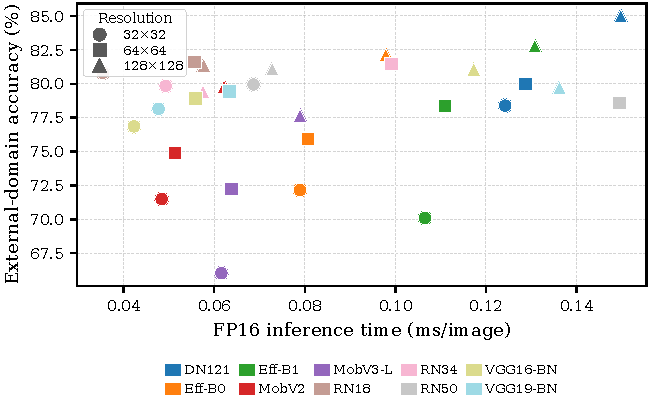
\includegraphics[width=\linewidth]{graphs/scatter_accuracy_latency}
  \caption{External accuracy vs.\ FP16 inference time.}
\end{subfigure}
\hfill
\begin{subfigure}[t]{0.31\linewidth}
  \centering
  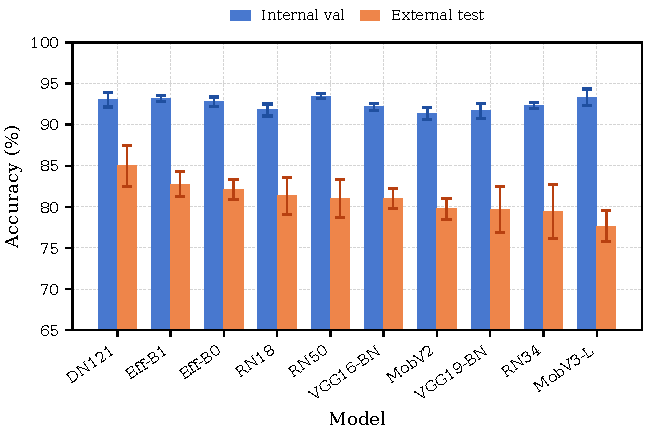
\includegraphics[width=\linewidth]{graphs/bar_domain_gap}
  \caption{Internal validation vs.\ external accuracy at 128$\times$128\,px.}
\end{subfigure}
\hfill
\begin{subfigure}[t]{0.31\linewidth}
  \centering
  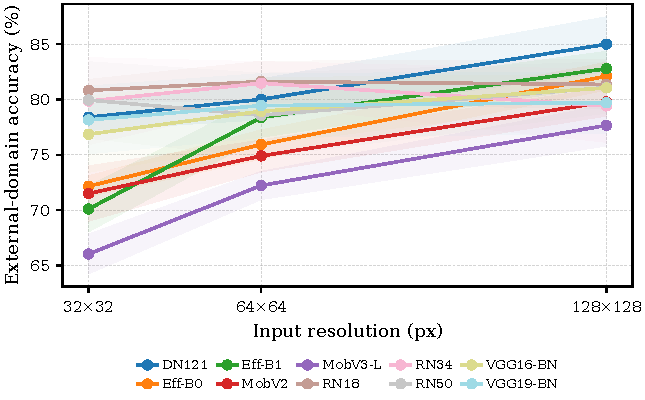
\includegraphics[width=\linewidth]{graphs/line_resolution_effect}
  \caption{Effect of input resolution on external accuracy.}
\end{subfigure}

\vspace{8pt}

\makebox[\linewidth][c]{%
\begin{subfigure}[t]{0.31\linewidth}
  \centering
  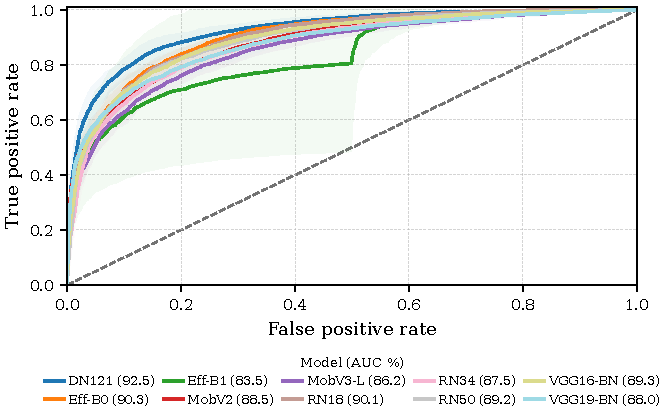
\includegraphics[width=\linewidth]{graphs/roc_curves_128x128}
  \caption{Mean ROC curves on the external test set at 128$\times$128\,px.}
\end{subfigure}
}

\caption{Cross-model summary of external-domain fire-detection performance. 
(a)~External accuracy versus FP16 inference time across models and resolutions. 
(b)~Internal validation versus external-test accuracy at 128$\times$128\,px. 
(c)~Resolution-wise external accuracy, reported as mean $\pm$ standard deviation over five runs. 
(d)~Mean ROC curves on the external test set at 128$\times$128\,px, with shaded regions showing $\pm$1 standard deviation.}

\label{fig:results_summary}
\end{figure*}





Figure~\ref{fig:results_summary} provides a four-panel visual summary of the key experimental outcomes, and the full numerical results are reported in Table~\ref{tab:internal_external_all_resolutions}. The sections below analyse each dimension in turn: cross-domain accuracy gaps, the effect of input resolution, the accuracy and latency trade-off, ROC discrimination, architectural latency drivers, and a comparison with prior published work.

\begin{table*}[!t]
\centering
\footnotesize
\caption{Internal-validation and external-domain performance comparison of all evaluated models across image resolutions.}
\label{tab:internal_external_all_resolutions}
\renewcommand{\arraystretch}{1.15}
\setlength{\tabcolsep}{3pt}
\resizebox{\linewidth}{!}{
\begin{tabular}{lcccccc}
\hline
\textbf{Model Name} & \textbf{Resolution} & \textbf{Val. Acc. (\%)} & \textbf{Ext. Acc. (\%)} & \textbf{AP (\%)} & \textbf{ROC-AUC (\%)} & \textbf{FP16 IT (ms)} \\
\hline
ResNet-18 & 32$\times$32 & 88.16 $\pm$ 1.08 & 80.81 $\pm$ 0.99 & 88.28 $\pm$ 1.39 & 88.25 $\pm$ 0.95 & \textbf{0.0354} \\
ResNet-18 & 64$\times$64 & 90.05 $\pm$ 0.63 & 81.61 $\pm$ 1.84 & 90.20 $\pm$ 1.63 & 89.96 $\pm$ 1.50 & 0.0556 \\
ResNet-18 & 128$\times$128 & 91.79 $\pm$ 0.73 & 81.36 $\pm$ 2.23 & 90.07 $\pm$ 2.29 & 90.14 $\pm$ 1.92 & 0.0576 \\
\hline
ResNet-34 & 32$\times$32 & 88.76 $\pm$ 0.69 & 79.84 $\pm$ 3.93 & 87.84 $\pm$ 4.05 & 87.97 $\pm$ 3.83 & 0.0493 \\
ResNet-34 & 64$\times$64 & 90.75 $\pm$ 1.08 & 81.46 $\pm$ 1.94 & 90.08 $\pm$ 2.02 & 90.00 $\pm$ 1.85 & 0.0991 \\
ResNet-34 & 128$\times$128 & 92.34 $\pm$ 0.41 & 79.41 $\pm$ 3.29 & 87.60 $\pm$ 2.39 & 87.46 $\pm$ 3.09 & 0.0575 \\
\hline
ResNet-50 & 32$\times$32 & 87.51 $\pm$ 0.54 & 79.95 $\pm$ 3.45 & 87.33 $\pm$ 2.96 & 87.58 $\pm$ 3.55 & 0.0687 \\
ResNet-50 & 64$\times$64 & 89.60 $\pm$ 0.48 & 78.57 $\pm$ 3.79 & 87.69 $\pm$ 3.52 & 86.82 $\pm$ 3.49 & 0.1495 \\
ResNet-50 & 128$\times$128 & \textbf{93.48 $\pm$ 0.32} & 81.07 $\pm$ 2.31 & 88.84 $\pm$ 1.37 & 89.21 $\pm$ 1.79 & 0.0728 \\
\hline
MobileNet-V2 & 32$\times$32 & 79.95 $\pm$ 1.82 & 71.49 $\pm$ 2.50 & 80.40 $\pm$ 3.33 & 78.71 $\pm$ 3.00 & 0.0484 \\
MobileNet-V2 & 64$\times$64 & 87.36 $\pm$ 1.10 & 74.89 $\pm$ 1.44 & 84.23 $\pm$ 1.43 & 83.47 $\pm$ 1.81 & 0.0513 \\
MobileNet-V2 & 128$\times$128 & 91.34 $\pm$ 0.71 & 79.78 $\pm$ 1.28 & 89.52 $\pm$ 0.94 & 88.47 $\pm$ 0.97 & 0.0622 \\
\hline
MobileNet-V3-Large & 32$\times$32 & 75.17 $\pm$ 1.84 & 66.03 $\pm$ 1.79 & 70.43 $\pm$ 2.38 & 72.13 $\pm$ 2.19 & 0.0616 \\
MobileNet-V3-Large & 64$\times$64 & 88.61 $\pm$ 0.64 & 72.22 $\pm$ 1.27 & 81.81 $\pm$ 1.08 & 80.37 $\pm$ 1.71 & 0.0639 \\
MobileNet-V3-Large & 128$\times$128 & 93.33 $\pm$ 1.02 & 77.65 $\pm$ 1.86 & 87.34 $\pm$ 1.95 & 86.23 $\pm$ 2.18 & 0.0790 \\
\hline
EfficientNet-B0 & 32$\times$32 & 79.25 $\pm$ 1.83 & 72.16 $\pm$ 0.93 & 78.88 $\pm$ 1.48 & 80.10 $\pm$ 1.14 & 0.0789 \\
EfficientNet-B0 & 64$\times$64 & 87.26 $\pm$ 0.59 & 75.93 $\pm$ 1.32 & 84.78 $\pm$ 0.83 & 84.22 $\pm$ 1.10 & 0.0807 \\
EfficientNet-B0 & 128$\times$128 & 92.79 $\pm$ 0.58 & 82.11 $\pm$ 1.25 & 90.49 $\pm$ 1.28 & 90.33 $\pm$ 1.12 & 0.0979 \\
\hline
EfficientNet-B1 & 32$\times$32 & 78.31 $\pm$ 1.22 & 70.09 $\pm$ 2.06 & 75.76 $\pm$ 2.76 & 77.62 $\pm$ 2.29 & 0.1065 \\
EfficientNet-B1 & 64$\times$64 & 88.66 $\pm$ 0.57 & 78.37 $\pm$ 1.79 & 88.10 $\pm$ 1.66 & 87.16 $\pm$ 1.65 & 0.1109 \\
EfficientNet-B1 & 128$\times$128 & 93.23 $\pm$ 0.37 & 82.78 $\pm$ 1.56 & 84.23 $\pm$ 15.06 & 83.50 $\pm$ 16.27 & 0.1308 \\
\hline
DenseNet-121 & 32$\times$32 & 87.11 $\pm$ 0.69 & 78.39 $\pm$ 1.19 & 87.45 $\pm$ 0.79 & 86.96 $\pm$ 0.92 & 0.1242 \\
DenseNet-121 & 64$\times$64 & 90.25 $\pm$ 0.69 & 80.00 $\pm$ 1.84 & 88.91 $\pm$ 1.29 & 88.53 $\pm$ 1.52 & 0.1287 \\
DenseNet-121 & 128$\times$128 & 93.03 $\pm$ 0.88 & \textbf{84.99 $\pm$ 2.48} & \textbf{92.49 $\pm$ 1.57} & \textbf{92.51 $\pm$ 1.73} & 0.1498 \\
\hline
VGG-16-BN & 32$\times$32 & 87.91 $\pm$ 0.80 & 76.85 $\pm$ 3.44 & 84.73 $\pm$ 3.58 & 84.84 $\pm$ 3.35 & 0.0423 \\
VGG-16-BN & 64$\times$64 & 90.40 $\pm$ 0.48 & 78.93 $\pm$ 3.03 & 87.01 $\pm$ 2.44 & 86.13 $\pm$ 2.85 & 0.0559 \\
VGG-16-BN & 128$\times$128 & 92.19 $\pm$ 0.42 & 81.04 $\pm$ 1.24 & 89.22 $\pm$ 1.55 & 89.29 $\pm$ 1.18 & 0.1173 \\
\hline
VGG-19-BN & 32$\times$32 & 87.61 $\pm$ 1.13 & 78.15 $\pm$ 3.06 & 85.43 $\pm$ 4.04 & 85.16 $\pm$ 3.41 & 0.0477 \\
VGG-19-BN & 64$\times$64 & 90.40 $\pm$ 0.54 & 79.44 $\pm$ 2.89 & 88.20 $\pm$ 2.33 & 87.00 $\pm$ 2.94 & 0.0634 \\
VGG-19-BN & 128$\times$128 & 91.69 $\pm$ 0.89 & 79.71 $\pm$ 2.79 & 89.10 $\pm$ 2.61 & 87.95 $\pm$ 2.39 & 0.1362 \\
\hline
\end{tabular}
}
\caption*{\footnotesize Note: Val. Acc. denotes internal validation accuracy, Ext. Acc. denotes external-domain test accuracy, AP denotes average precision, ROC-AUC denotes receiver operating characteristic area under the curve, and IT denotes inference time per image. Bold values indicate the best result in each column; for FP16 IT, the lowest value is bolded.}
\end{table*}

\subsection{Evaluation Protocol}

The full training and evaluation pipeline is shown in Figure~\ref{fig:pipeline}, and the same training settings were applied to all 150 configurations. All experiments ran on an NVIDIA GeForce RTX~5090 GPU. Ten architectures were evaluated at three resolutions (32$\times$32, 64$\times$64, and 128$\times$128\,px) under five random seeds. Per-image FP16 inference time was measured at batch size~32 with PyTorch automatic mixed precision on the external test set. For each configuration, the checkpoint with the highest internal validation accuracy was used for both internal and external evaluation, so all reported numbers reflect the best-generalising state rather than the final epoch.

\subsection{Internal and External-Domain Performance}

A central result is the consistent, often large gap between internal validation accuracy and external accuracy, seen most clearly in Figure~\ref{fig:results_summary}(b) at 128$\times$128. On the internal split, ResNet-50 leads with \textbf{93.48$\pm$0.32\%}, ahead of MobileNet-V3-Large (93.33$\pm$1.02\%), EfficientNet-B1 (93.23$\pm$0.37\%), and DenseNet-121 (93.03$\pm$0.88\%). This near-parity hides sharply different behaviour on the external forest fire domain.

MobileNet-V3-Large, second internally, falls to \textbf{77.65$\pm$1.86\%} externally, a drop of 15.7 points and the largest at this resolution. ResNet-50 declines from 93.48\% to 81.07$\pm$2.31\% despite its top validation score. DenseNet-121 shows the smallest gap among the strong models: its external accuracy of \textbf{84.99$\pm$2.48\%} is only 8.0 points below its validation figure, and it also attains the highest average precision (\textbf{92.49$\pm$1.57\%}) and ROC-AUC (\textbf{92.51$\pm$1.73\%}) on the external set. The bar heights in Figure~\ref{fig:results_summary}(b) make the pattern clear: a model that fits its training distribution tightly can still generalise poorly when scene composition, acquisition conditions, or environment change, so internal accuracy is an unreliable proxy for external performance. Figure~\ref{fig:dataset_samples} shows why: the wildfire domain has denser smoke and darker tones, while the forest fire images show lighter flames against open canopy, a shift that calls for domain-invariant features and accounts for the failures.

\subsection{Effect of Input Resolution on Cross-Domain Accuracy}

Figure~\ref{fig:results_summary}(c) plots external accuracy against input resolution for all ten architectures. For most, accuracy rises monotonically from 32$\times$32 to 128$\times$128. The largest gain is DenseNet-121's, from 78.39$\pm$1.19\% to \textbf{84.99$\pm$2.48\%} (6.6 points), as higher resolution preserves flame texture, smoke boundaries, and background structure. EfficientNet-B0 rises similarly, from 72.16$\pm$0.93\% to 82.11$\pm$1.25\% (nearly 10 points), and MobileNet-V2 (71.49\%\,$\to$\,79.78\%) and VGG-16-BN (76.85\%\,$\to$\,81.04\%) gain steadily.

The trend is not universal. ResNet-34 peaks at 64$\times$64 (81.46$\pm$1.94\%) and drops to 79.41$\pm$3.29\% at 128$\times$128 with higher variance, suggesting its residual features gain little from, and may be hindered by, the extra high-frequency texture at full resolution under domain shift. ResNet-18 saturates above 64$\times$64 (80.81\%\,$\to$\,81.61\%\,$\to$\,81.36\%), showing diminishing returns for this lightweight backbone. Resolution is therefore an architecture-specific choice: whether more spatial detail helps under domain shift depends on each family's inductive biases.

\subsection{Accuracy and Latency Trade-Off}

Figure~\ref{fig:results_summary}(a) plots all 30 model-resolution configurations as external accuracy versus FP16 inference time, revealing a clear Pareto frontier. The fastest is ResNet-18 at 32$\times$32 at \textbf{0.0354\,ms} per image, roughly four times faster than most mid-range configurations, while still reaching 80.81$\pm$0.99\% external accuracy. Along the frontier, ResNet-18 at 64$\times$64 gives 81.61$\pm$1.84\% at 0.0556\,ms, a useful gain for a 57\% rise in latency, and EfficientNet-B0 at 128$\times$128 sits at 82.11$\pm$1.25\% and 0.0979\,ms. At the top, DenseNet-121 at 128$\times$128 reaches \textbf{84.99$\pm$2.48\%} at 0.1498\,ms, the second-highest latency in the benchmark, with the best AP and AUC in Table~\ref{tab:internal_external_all_resolutions}.

Resolution scaling does not help every model equally. For ResNet-18, moving from 32$\times$32 to 128$\times$128 barely changes accuracy yet raises latency by 63\%; for EfficientNet-B0, the same step adds nearly 10 points of accuracy for only a 24\% latency increase, a far better exchange. Resolution should therefore be chosen with both architecture and latency budget in mind, not fixed at the largest available size.

\subsection{Cross-Domain Discrimination and ROC Analysis}

Figure~\ref{fig:results_summary}(d) overlays the mean ROC curves of all ten architectures at 128$\times$128 on the external set, with bands showing $\pm$1 standard deviation across five runs. Every model lies well above the chance diagonal, so fire/no-fire discrimination is tractable across architectures at this resolution. DenseNet-121 has the highest mean AUC (\textbf{92.51$\pm$1.73\%}), consistent with its accuracy; EfficientNet-B0 follows at 90.33$\pm$1.12\%, and ResNet-18 reaches a strong 90.14$\pm$1.92\% for a lightweight backbone. The narrow bands on most curves indicate stable behaviour across seeds.

EfficientNet-B1 at 128$\times$128 is the exception: its AUC and AP spreads ($\pm$16.27\% and $\pm$15.06\%) dwarf those of any other configuration, indicating unstable training or high sensitivity to initialization that the mean accuracy hides. MobileNet-V3-Large reaches only 86.23$\pm$2.18\% AUC externally despite its strong validation score, confirming its tendency to overfit the training domain. Overall, the ROC curves confirm DenseNet-121 as the most reliable external discriminator and show that per-seed AUC variance reveals stability information that accuracy alone does not.

\subsection{Architectural Factors Governing Mixed-Precision Latency}

The FP16 inference times in Table~\ref{tab:internal_external_all_resolutions} follow each architecture's structure rather than its parameter count. ResNet-18 (11.17 million parameters) is fastest at 0.0354\,ms (32$\times$32) because its shallow residual blocks use element-wise additions with regular memory access that maps efficiently onto half-precision Tensor Core operations. DenseNet-121, with only 7.98 million parameters, still needs 0.1498\,ms at 128$\times$128: its dense connectivity repeatedly concatenates feature maps from all earlier layers, raising memory-bandwidth demand and breaking the contiguous access that FP16 throughput depends on.

EfficientNet-B0 and B1 use depthwise separable convolutions under compound scaling; these cut floating-point operations but their irregular memory access raises latency relative to parameter count compared with ResNet-18. The effect is visible in the data: EfficientNet-B0 at 128$\times$128 runs at 0.0979\,ms for 82.11\% accuracy, while ResNet-18 at 64$\times$64 runs at 0.0556\,ms for 81.61\%, a 43\% latency reduction for a 0.50-point accuracy cost. MobileNet-V3-Large adds squeeze-and-excitation modules whose sequential channel dependencies push its latency to the level of deeper ResNet variants at the same resolution. For FP16 deployment, then, architectures with regular parallel memory patterns and shallow skip connections are most latency-efficient, while dense connectivity and channel attention carry a cost that must be repaid in accuracy.

\begin{table*}[t]
\footnotesize
\setlength{\tabcolsep}{3pt}
\caption{Performance comparison of representative fire detection models
across accuracy and inference time metrics, including cross-domain
evaluation results at multiple input resolutions}
\centering
\resizebox{\linewidth}{!}{
\begin{tabular}{|l|c|c|c|c|c|c|}
\hline
\textbf{Model Name}
  & \textbf{Accuracy (\%)}
  & \textbf{Precision}
  & \textbf{Recall}
  & \textbf{Parameters (M)}
  & \textbf{GFLOPs}
  & \textbf{Inference Time (ms)} \\
\hline
CNN~\cite{muhammad2018efficient}
  & 92.04 & 0.90 & 0.93 & {--} & {--} & 43.68 \\
Faster R-CNN~\cite{chaoxia2020information}
  & 93.36 & 0.95 & 0.92 & {--} & {--} & 46.30 \\
EfficientNetB0-HDA~\cite{elmadafri2024dual}
  & 95.36 & 0.96 & 0.96 & 4.05 & {--} & 5.46\textsuperscript{a} \\
YOLOv4-EfficientNetV2-ECA~\cite{mamadmurodov2025hybrid}
  & 93.13\textsuperscript{b} & 0.97 & 0.95 & {--} & {--} & 27.0\textsuperscript{a} \\
MobileNetV2~\cite{mambile2025cnn}
  & 99.00 & 0.99 & 0.99 & 3.5 & {--} & 12.0\textsuperscript{a} \\
IRTQ~\cite{bukhari2025irtq}
  & 98.90 & 0.99 & 0.99 & 0.09 & {--} & 3.0\textsuperscript{a} \\
\hline
\textbf{DenseNet-121 (128$\times$128)} -- Val.
  & 93.03\,$\pm$\,0.88 & {--} & {--} & 7.98 & {--} & {0.1498} \\
\textbf{DenseNet-121 (128$\times$128)} -- Ext.\textsuperscript{c}
  & \textbf{84.99\,$\pm$\,2.48} & {--} & {--} & 7.98 & {--} & {0.1498} \\
ResNet-18 (32$\times$32) -- Val.
  & 88.16\,$\pm$\,1.08 & {--} & {--} & 11.17 & {--} & \textbf{0.0354} \\
ResNet-18 (32$\times$32) -- Ext.\textsuperscript{c}
  & 80.81\,$\pm$\,0.99 & {--} & {--} & 11.17 & {--} & \textbf{0.0354} \\
\hline
\multicolumn{7}{|l|}{%
\footnotesize
\textsuperscript{a}Inference time reported on different hardware;
not directly comparable to our FP16 latency on RTX\,5090.} \\
\multicolumn{7}{|l|}{%
\footnotesize
\textsuperscript{b}Reported as mAP; per-class classification
accuracy not stated in the original work.} \\
\multicolumn{7}{|l|}{%
\footnotesize
\textsuperscript{c}Ext. denotes external-domain test accuracy
on a separate forest fire dataset unseen during training
(5-seed mean\,$\pm$\,std).} \\
\multicolumn{7}{|l|}{%
\footnotesize
Our inference time: per-image FP16 latency, batch size\,=\,32.
Precision/Recall not reported; evaluation uses AUC-based metrics.} \\
\hline
\end{tabular}
}
\label{tab:Model_Comparison}
\end{table*}

\subsection{Comparison with Prior Work}

Table~\ref{tab:Model_Comparison} places our best configurations beside representative published models. Those methods report 92.04\% to 99.00\% accuracy, well above our best external accuracy of 84.99\%, but the comparison is not like-for-like: each cited system is tested on an internal set from its own training distribution, whereas our external accuracy comes from a separate dataset never seen during training, and in-distribution testing almost always scores higher than cross-domain testing. For a fair point of contact, our DenseNet-121 at 128$\times$128 reaches 93.03\% on its internal validation split, comparable to several of these baselines, while still holding 84.99\% under the harder external condition. The high figures of MobileNetV2~\cite{mambile2025cnn} (99.00\%) and IRTQ~\cite{bukhari2025irtq} (98.90\%) thus reflect favourable in-distribution conditions rather than cross-domain capability, a distinction that matters for real deployment.

Latency is also not directly comparable, since prior timings are reported on CPUs or unspecified GPUs (footnote~\textsuperscript{a} in Table~\ref{tab:Model_Comparison}). Even so, our fastest configuration, ResNet-18 at 32$\times$32 (0.0354\,ms/image), falls well below the times of EfficientNetB0-HDA~\cite{elmadafri2024dual} (5.46\,ms), IRTQ~\cite{bukhari2025irtq} (3.0\,ms), and the CNN baseline of Muhammad~et~al.~\cite{muhammad2018efficient} (43.68\,ms), even allowing for hardware differences. This gap reflects the efficiency of half-precision computation on modern GPUs and shows that mixed-precision inference is a practical route to real-time fire detection without loss of accuracy.

\subsection{Model Selection Guidelines}

The results support three deployment recommendations. \textbf{For maximum cross-domain robustness}, such as high-stakes UAV surveys or alerting systems where test conditions differ greatly from training, DenseNet-121 at 128$\times$128 is preferred, giving \textbf{84.99$\pm$2.48\%} external accuracy, \textbf{92.49$\pm$1.57\%} AP, \textbf{92.51$\pm$1.73\%} AUC, at 0.1498\,ms per image. \textbf{For latency-constrained edge use}, such as onboard UAV processors, embedded cameras, or IoT nodes, ResNet-18 at 32$\times$32 gives the lowest FP16 latency (0.0354\,ms) at 80.81$\pm$0.99\% accuracy, and ResNet-18 at 64$\times$64 raises this to 81.61$\pm$1.84\% for a 57\% latency increase. \textbf{For a balance of accuracy and speed}, EfficientNet-B0 at 128$\times$128 offers 82.11$\pm$1.25\% accuracy and 90.33\% AUC at 0.0979\,ms. In every case, external-domain evaluation is a necessary complement to internal validation when choosing a fire-detection model.


\section{Conclusion}

This study evaluated ten CNN architectures for binary fire/no-fire classification across two domains, three input resolutions (32$\times$32, 64$\times$64, and 128$\times$128\,px), and five seeds, giving 150 trained configurations. By separating training and internal testing from a fully independent external domain, the forest fire dataset, the design measures cross-domain generalisation rather than in-distribution fit. Per-image FP16 inference time under automatic mixed precision adds a practical dimension that prior comparisons rarely report.

The central finding is the gap between internal validation and external performance. At 128$\times$128 the top four architectures fall within 0.5 percentage points on internal validation, led by ResNet-50 (93.48$\pm$0.32\%), but this parity does not survive domain shift: MobileNet-V3-Large drops 15.7 points to 77.65$\pm$1.86\%, and ResNet-50 falls to 81.07$\pm$2.31\%. DenseNet-121 generalises best, holding 84.99$\pm$2.48\% external accuracy with the leading average precision (92.49$\pm$1.57\%) and ROC-AUC (92.51$\pm$1.73\%). The model with the highest internal accuracy is therefore not the most reliable in deployment, and external-domain evaluation is essential to any rigorous fire-detection study.

Higher resolution helps some architectures but not all. DenseNet-121 and EfficientNet-B0 improve steadily across the range (gains of 6.6 and 9.95 points), as finer detail preserves the flame texture and smoke boundaries useful for cross-domain discrimination, whereas ResNet-34 peaks at 64$\times$64 and regresses at 128$\times$128 with rising variance, and ResNet-18 saturates beyond 64$\times$64. The accuracy and latency scatter clarifies the trade-off: ResNet-18 at 32$\times$32 sets the speed frontier (0.0354\,ms, 80.81$\pm$0.99\%), EfficientNet-B0 at 128$\times$128 offers a balanced point (82.11$\pm$1.25\%, 0.0979\,ms), and DenseNet-121 at 128$\times$128 the accuracy ceiling (84.99$\pm$2.48\%, 0.1498\,ms). These differences are structural: ResNet-18's shallow residual blocks allow contiguous half-precision memory access, while DenseNet-121's feature-map concatenation raises bandwidth demand, a cost justified for accuracy-critical use by its stronger generalisation.

At 128$\times$128 every architecture discriminates well on the external domain, with all mean ROC curves above the chance diagonal and DenseNet-121 highest at 92.51$\pm$1.73\% AUC. The exception is EfficientNet-B1, whose AUC and AP spreads ($\pm$16.27\% and $\pm$15.06\%) far exceed any other configuration and indicate training instability that mean accuracy hides. Per-seed AUC variance is thus a more sensitive reliability diagnostic than mean accuracy and should be reported routinely in such benchmarks.

Several directions follow from this work. The benchmark should be extended to more fire datasets covering different regions, seasons, vegetation, and imaging altitudes, to test whether the cross-domain findings hold more broadly. Temporal models that use video, optical flow, or multi-frame inputs suit real-time alarms, where smoke and flame evolve across frames in ways static classifiers cannot exploit. Multispectral and thermal imagery would extend detection to dense smoke and night-time conditions that degrade visible-spectrum models, and would reveal whether the present rankings transfer. Moving from image-level classification to object detection and segmentation would add spatial localisation and test whether the same architectural ordering holds for that harder task. Domain-adaptation methods such as adversarial feature alignment, style-transfer augmentation, and test-time adaptation offer a route to narrowing the internal-to-external gap reported here. Finally, deployment benchmarking on embedded GPUs, UAV processors, and mobile edge accelerators would translate the FP16 latency figures into real power, memory, and thermal budgets for field use.





\bibliographystyle{IEEEtran}
\bibliography{references}

\end{document}
